%
% $Id: ch03_thework.tex
%
%   *******************************************************************
%   * SEE THE MAIN FILE "AllegThesis.tex" FOR MORE INFORMATION.       *
%   *******************************************************************
%
\chapter{Method of Approach} \label{ch:method}
In this chapter, we discuss the implementation details for our system.  The
implementation can be broken into four distinct sections:

\begin{enumerate}
\item XML parsing
\item Intermediate representation
\item Simplified representation
\item Risk evaluation
\end{enumerate}

\section{XML Parsing} \label{sec:parse}

When CodeCover produces per-test coverage information, it stores the results in
a container.  Though CodeCover features several coverage report export types, 
including hierarchical HTML, these reports do not include all of the information
necessary for this project.  Specifically, these export formats only include
general per-test coverage information, displaying percent coverage for each test.
They do not include information related to precisely which tests executed each 
statement, which is a requirement for suspiciousness analysis.  

Due to the limitations in CodeCover export formats, we are forced to make use of
the more complex XML container.  Since the container is in XML format, we must
first parse the file before we can perform analysis.  To that end, we utilize
DOM (document object model) parsing to store the entire container as a tree structure.  
We chose DOM over SAX (simple API for XML) due to the complexity of the container file.
Since SAX does not store the document in memory in its entirety, multi-pass analysis
is both more efficient and less complex when using DOM parsing.

\section{Intermediate Representation} \label{sec:ir}

After DOM parsing is complete, provided no errors occurred, the document tree root is
passed into the intermediate representation constructor.  The IR (intermediate representation)
for the container is designed to be simple to build while traversing a DOM of a CodeCover
container.  The \texttt{ContainerIR} object contains a list of \texttt{TestFile}s, as well
as a list of \texttt{String} names of test cases.  The object also includes boolean values,
in which the $i^{th}$ element indicates the pass/fail status of the $i^{th}$ test case.  A 
visualization of the container IR, as well as its internal data structures, can be found in 
Figures \ref{fig:ir} and \ref{fig:ir2}, respectively.  

\begin{figure}[tb]
\centering
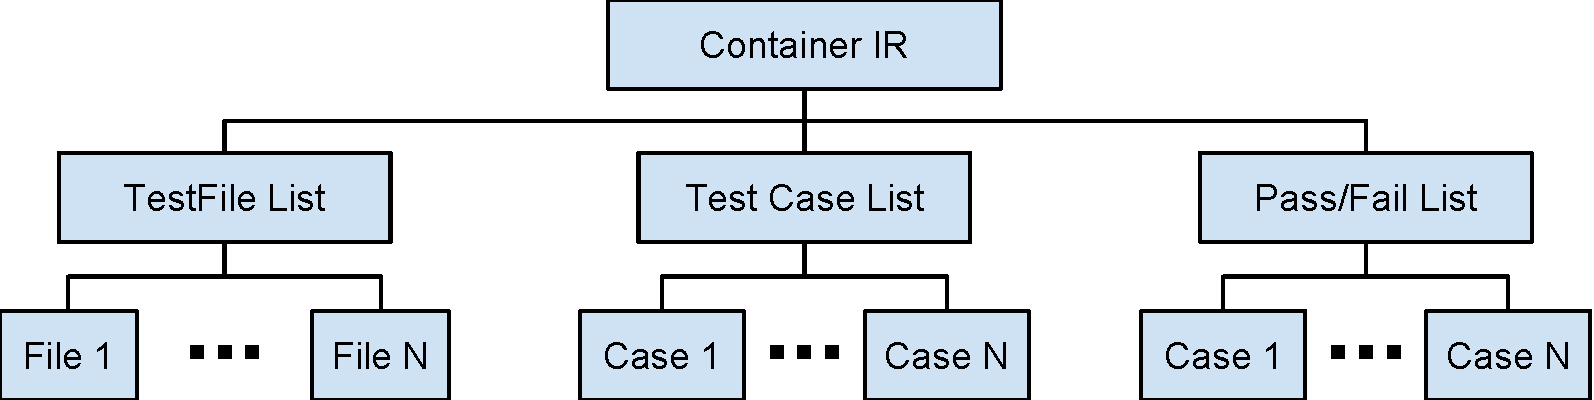
\includegraphics[width=0.8\linewidth]{img/ContainerIR.pdf}
\caption{Diagram of data structure for IR.}
\label{fig:ir}
\end{figure}

\begin{figure}[tb]
\centering
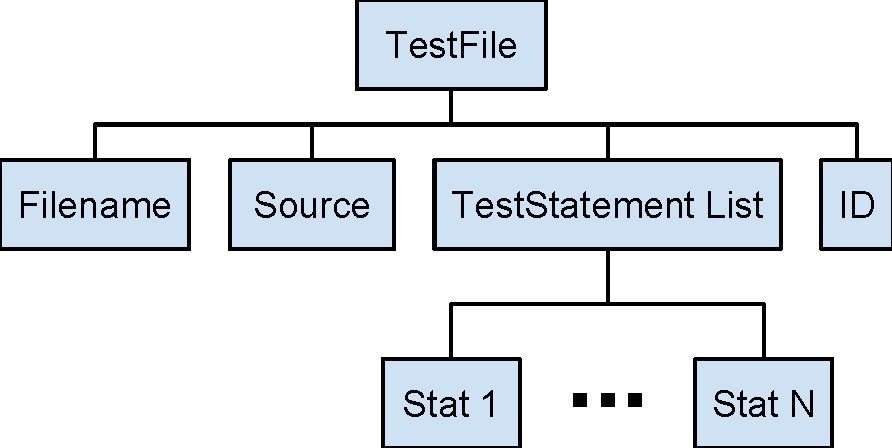
\includegraphics[height=30mm]{img/TestFile.pdf}
\hspace{0.1\linewidth}
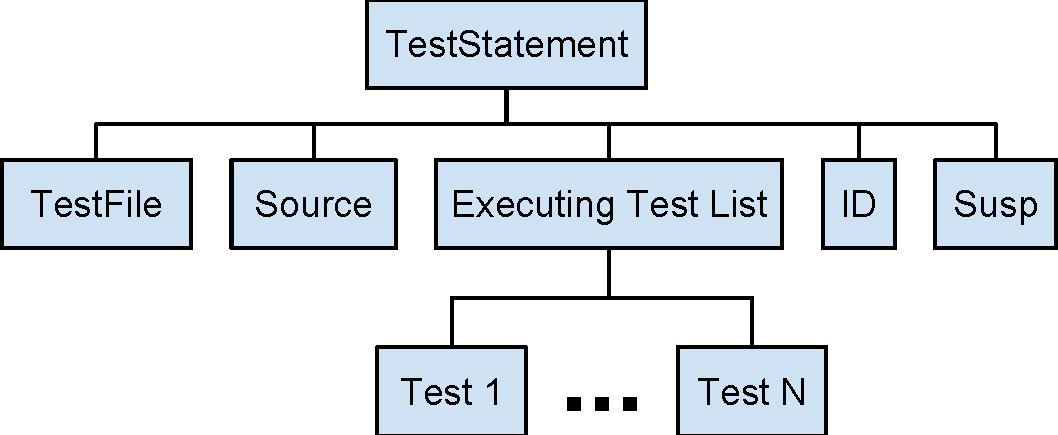
\includegraphics[height=30mm]{img/TestStatement.pdf}
\caption{Diagram of data structures used within the IR to store files (left) and 
statements (right).}
\label{fig:ir2}
\end{figure}

Each \texttt{TestFile} object contains the name and source code of the file as \texttt{String}s, the internal identification number for the file as an \texttt{int}, and a list of \texttt{TestStatement}s.  
A \texttt{TestStatement} includes an ID and source code for the statement, each stored as \texttt{String}s.  In addition, the \texttt{TestStatement} object stores a \texttt{TestFile} 
parent object and the suspiciousness value associated with the statement.  Finally, the statement 
includes a \texttt{boolean} list, where each element corresponds to a test case.  These boolean 
values indicate whether the respective test case executed this statement.  A \texttt{TestStatement} 
can be uniquely identified by the combination of its source file and ID.

CodeCover coverage containers include all required
information, divided into three sections.  First, the container lists all source
files included in coverage analysis, including the entirety of their source code,
the name of the file, and a unique internal identification value.  Following the source files
is a hierarchical list of all statements within those files.  These statements are defined by 
their category, source file, and character offset within the source file.  For this
project, we only consider basic statements---in Java, this essentially refers to executable
statements terminated with semicolons.  

The final section of a CodeCover container is the per-test coverage data itself.  This is
represented by a series of test cases, each of which contains a child for every file
executed by that test. Under each file is a list of specific statements executed by that
test inside that file.  These statements are identified by their alphanumeric identifier.

Our system processes these sections in the order they appear above.  Using the DOM produced
from parsing, we can easily traverse the relevant segments of the container.  Traversal of
the DOM tree consists of repeated iterations of sub-levels of the XML hierarchy in order
to locate a node with a specific name.  Throughout this process, we make no assumptions about
the sequence in which nodes appear.  For example, rather than assuming a given node is
always the first child, we always use a loop structure to make certain we identify the correct
node.

In order to identify all source files defined by the
XML container, we first locate the \texttt{SrcFileList} node.  We then iterate through its
children to locate all \texttt{SrcFile} nodes.  For each \texttt{SrcFile} node found, we 
extract the attributes of that node and add a \texttt{TestFile} to the \texttt{ContainerIR}
file list.  

Once we have located the source files, we must identify the statements.  To do so, we first
locate the hierarchical statement definition root.  Beginning with that root node, we recursively
traverse the entire sub-tree.  Within the hierarchical component of a CodeCover container there
exists a \texttt{BasicStmnt} node, demonstrated by the excerpt shown in Figure \ref{fig:xml-basic}, for every basic statement in the source code.  For each \texttt{BasicStmnt} node, we add a new statement to the 
correct \texttt{TestFile}.  In order to do so, we must first identify the \texttt{LocList} child
node, followed by its \texttt{Loc} child node.  The attributes of the \texttt{Loc} node include
the source code character offset for the basic statement in question.  Between the attributes of
the \texttt{BasicStmnt} node and those of the \texttt{Loc} node, we extract the information
necessary to create a new \texttt{TestStatement} object.  Once this recursive traversal of the
statement hierarchy is complete, the \texttt{TestFile}s in the \texttt{ContainerIR} will contain
all basic statements.

\begin{figure}[tb]
\centering
\begin{lstlisting}
<BasicStmnt CovItemId="S19" 
	CovItemPrefix="net.sf.jniinchi.JniInchiStructure.java"
	Intrnl_Id="457">
		<LocList>
				<Loc EndOffset="3716" SrcFileId="4" StartOffset="3672"/>
		</LocList>
</BasicStmnt>
\end{lstlisting}

\caption{Excerpt of a container showing a single \texttt{BasicStmnt} element.  This excerpt is taken
from the CodeCover container produced from the Jni-Inchi case application.  The statement defined here
has the ID \texttt{S19} and consists of the source code from character position \texttt{3672} to 
\texttt{3716} within the file with name \texttt{net.sf.jniinchi.JniInchiStructure.java}.}
\label{fig:xml-basic}
\end{figure}

Since we now have a complete list of basic statements, we can process the coverage data section
of the container to identify test cases and their coverage.  To begin, we first iteratively 
locate the \texttt{TestSession} node, whose children include a \texttt{TestCase} node for
each test case in the test suite.  We add the name of each test case to the \texttt{ContainerIR}
test case list, then process the children of the node to find coverage data.  Each test case
node contains a hierarchy of \texttt{CovList}, \texttt{CovPrefix}, and \texttt{Cov} nodes.  We 
locate all \texttt{CovPrefix} nodes, which each correspond to a single file, then retrieve the
\texttt{TestFile} corresponding to this node from the list of test files within the \texttt{ContainerIR}.
Finally, we iterate through all \texttt{Cov} children of the \texttt{CovPrefix} to find all 
basic statements covered by a given test case within a given file.  For each statement identified,
we mark the corresponding \texttt{TestStatement} as covered.

In addition to coverage data, a \texttt{TestCase} node also contains a \texttt{Comment} attribute.
The content of this attribute is comprised of the entire text output produced when the test case
was executed.  When the test case passes, this attribute is empty; however, when a failure occurs,
the description of the failure is stored in this node.  As a result, we can observe this attribute
to determine the pass/fail status of a given test.  We ascertain this data by checking the
\texttt{Comment} attribute for the starting string \texttt{"Failure"}.  Since this word always
heads the description of a failure, the \texttt{Comment} of a failed test will always begin with
the same text.  We also allow the text \texttt{"Error"} to indicate a failing test, since an unhandled
error in a test case indicates that the test did not complete successfully.  This pass/fail value is
recorded in the boolean list stored in the \texttt{ContainerIR}, where true indicates a passed test and
false indicates a one in which a failure occurred.

\section{Simplified Representation} \label{sec:sir}

The intermediate representation discussed in Section \ref{sec:ir} is appropriate as a preliminary
data structure.  However, it is not conducive to suspiciousness analysis.  All of the risk evaluation
functions considered in this project require four pieces of information for each statement that
must be evaluated: $ae_f, ae_p, an_f, \text{ and } an_p$ \cite{theory}.  These variables represent the number
of test cases that meet certain requirements for a given statement, defined below:

\begin{itemize}
\item $ae_f$:  Number of test cases that execute the statement and fail.
\item $ae_p$:  Number of test cases that execute the statement and pass.
\item $an_f$:  Number of test cases that do NOT execute the statement and fail.
\item $an_p$:  Number of test cases that do NOT execute the statement and pass.
\end{itemize}

These four values become the input to each of
the suspiciousness functions.  Therefore, the simplified representation (SR) that best suits our needs
is one that stores these values for each statement, with no extraneous information.

\begin{figure}[tb]
\centering
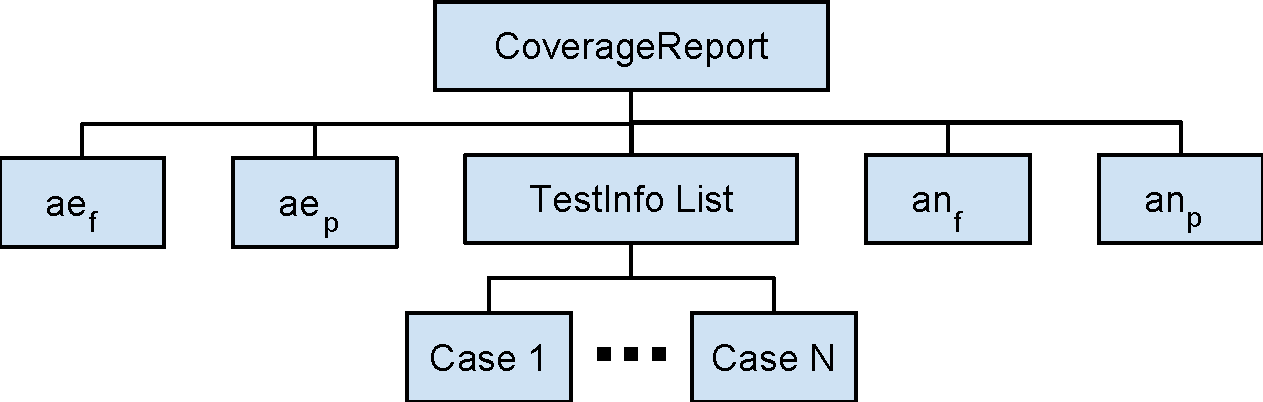
\includegraphics[height=28mm]{img/CoverageReport.pdf}
\hspace{0.1\linewidth}
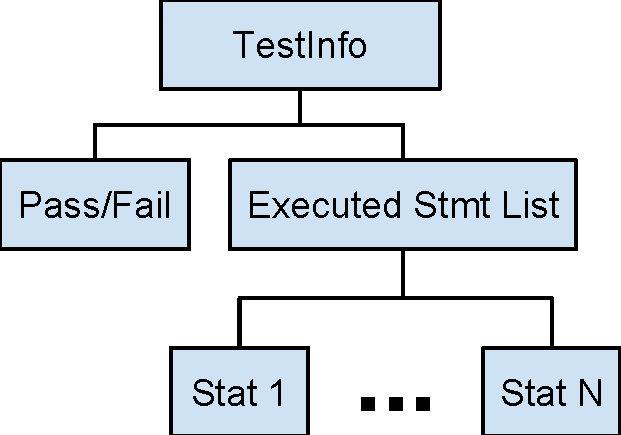
\includegraphics[height=28mm]{img/TestInfo.pdf}
\caption{Diagram of data structures for simplified representation (left) and  storing information
about a single test case within the SR (right).}
\label{fig:sr}
\end{figure}

In order to convert the IR to the described simple representation, the first step is to build
a list of \texttt{TestInfo} objects, which represent individual test cases.  Each \texttt{TestInfo}
object includes a pass/fail boolean value, as well as a boolean list that describes, for each
statement under test, whether that statement was executed by this test.  A visualization of this
data structure can be found in Figure \ref{fig:sr}. We extract this information 
from the IR by iterating through the list of test case names.  For each test case, we check the
execution status of that test case for each statement, storing this information in a list (where
each element corresponds to a single statement and true indicates the statement was executed by this
test).  Next, we cross check that test case index with the corresponding element in the pass/fail
boolean list in the IR and set the pass/fail status of the new \texttt{TestInfo} object to reflect
that value.


Iterating through the \texttt{TestInfo} list, we can determine the $ae_f, ae_p, an_f, \text{ and } an_p$
of each statement.  For each test case, we check whether the test passed then determine which statements
it executed by iterating through the boolean list stored in the \texttt{TestInfo} object.  For each
statement, we increment the appropriate variable depending on its pass/fail and execution status.  The
result is a list---for each of the four variables---in which each element corresponds to its value for
the corresponding statement.  After completing this process, we have a \texttt{CoverageReport} object
with all of the information necessary for risk evaluation.  This data structure is demonstrated by the 
diagram in Figure \ref{fig:sr}.

\section{Risk Evaluation} \label{sec:re}

There are many different risk evaluation functions, but all of those studied here are structurally similar.  We internally
represent risk evaluation functions using our \texttt{REFunction} interface.  This interface provides
abstract methods for returning the name of the function and for evaluating the function on provided
$ae_f, ae_p, an_f, \text{ and } an_p$.  Figure \ref{fig:re} provides an example implementation of
the REFunction interface.  For each function included, we create an implementation of
\texttt{REFunction}.  A complete list of \texttt{REFunctions} is stored in a static array of the
same name in \texttt{CoverageReport} for ease of iteratively performing all evaluation functions.  The
risk evaluation functions studied are listed in Table \ref{tab:ref}.

\begin{table}[tb]
\centering
{\renewcommand{\arraystretch}{2}
\begin{tabular}{|c|c|}\hline
Name & Formula expression\\\hline
Tarantula & $\displaystyle{\frac{a_{ef}}{a_{ef} + a_{nf}} / \left( \frac{a_{ef}}{a_{ef} + a_{nf}} + \frac{a_{ep}}{a_{ep} + a_{np}}\right)}$\\\hline
Jaccard & $\displaystyle{\frac{a_{ef}}{a_{ef} + a_{nf} + a_{ep}}}$\\\hline
Kulczynski2 & $\displaystyle{\frac{1}{2}\left( \frac{a_{ef}}{a_{ef} + a_{nf}} + \frac{a_{ef}}{a_{ef} + a_{np}} \right)}$\\\hline
Ochiai & $\displaystyle{ \frac{a_{ef}}{\sqrt{(a_{ef} + a_{nf})(a_{ef} + a_{ep})}}}$\\\hline
AMPLE2 & $\displaystyle{ \frac{a_{ef}}{a_{ef} + a_{nf}} - \frac{a_{ep}}{a_{ep} + a_{np}} }$\\\hline
\end{tabular}}
\caption{Complete list of risk evaluation functions studied in this project.}
\label{tab:ref}
\end{table}

\begin{figure}[tb]
\centering
\begin{lstlisting}
public class Jaccard implements REFunction {
	public double analyze( int aef, int aep, int anf, int anp ) {
		return ( (double) aef / (aef + anf + aep ) );
	}

	public String toString() {
		return "Jaccard";
	}
}
\end{lstlisting}

\caption{Implementation of REFunction interface for Jaccard function.}
\label{fig:re}
\end{figure}

When performing risk evaluation, we iterate through the specified functions.  For each of these
functions, we store the results of analysis in a \texttt{ResultsList} data structure.  This
structure allows for ease of sorting analyzed statements by suspiciousness rating.  In addition, the
suspiciousness values of the \texttt{ResultsList} are normalized to a zero-to-one scale according to

\[ L_i = \frac{ L_i - L_{min} }{ L_{max} - L_{min} }. \]

In this equation, $L_i$ refers to the $i^{th}$ element of the \texttt{ResultsList}, and $L_{max}, L_{min}$
refer to the maximum and minimum values in the list, respectively.  Though normalizing the results does
not change the ordering of the statements, it does make the actual suspiciousness values easier to compare
across multiple different functions.  The final result of analysis is a list of statements, ordered from
most suspicious to least suspicious, with values ranging from zero (not suspicious) to one (very 
suspicious).  In the case of undefined results to risk evaluation functions (specifically, any time a
risk evaluation function returns \texttt{NaN}), we treat the value as zero.  This avoids problems such as
completely uncovered statements always appearing as the most suspicious value.

\section{Overview} \label{sec:over}

When executing the system, the main class, \texttt{Test.java}, must be invoked with three additional
parameters:

\begin{enumerate}
\item Name of the CodeCover container to be analyzed.  Only the filename, not the path, should be included.  The file must be placed in the \texttt{containers/} directory.
\item Output file name.  This should be the name of the case application being studied.  The file will be placed in the (to be created) \texttt{results/} directory.
\item Source code of faulty statement inserted into the case application.
\end{enumerate}

Execution begins with parsing the XML container.  When the document has been stored as a DOM, it is
passed forward to the \texttt{ContainerIR} constructor, which processes the document into an IR as
described previously.  The IR is then passed to the \texttt{CoverageReport} class, where the 
test class is executed and coverage information is collated into the simple representation.
Suspiciousness evaluation is then completed using all of the risk evaluation functions specified.

After performing suspiciousness evaluation, the results are written to CSV (comma
separated value) format output file.  The attributes \textit{Function, Statement ID, Filename, Suspiciousness, Rank,
Statement Count, Case Application,} and \textit{IsFault} serve to uniquely identify a statement 
while providing information on risk evaluation.  The \textit{IsFault} field is always either true or 
false and is produced by comparing the source of each statement to the provided faulty statement. 
If these statements match, true will be written; otherwise, false is written.
This format conforms to the \textit{tidy data} \cite{tidy} standard, a ``standard way of mapping the meaning of a 
dataset to its structure'', in that each variable forms a column and each observation forms a row.  
This organizational structure allows for reliably simple evaluation of data using statistical 
analysis tools.  Though tidy data contains extensive redundancy, that redundancy simplifies
the data analysis and visualization process.